%%%%%%%%%% NO OLVIDAR COLOCAR ESTE COMENTARIO CON EL NUMERO DE EJERCICIO %%%%%%%%%%%%%
%%%%%%%%%%%%%%%%%%% EJERCICIO 9 %%%%%%
%%Text bf para negrilla , el \\ es para el salto de linea.
%%El primer \\ hace un espacio en el texto y el 2 \\ crea otro espacio
\textbf{Ejemplo 7}\newline
Elaborar una tabla para amortizar la suma de 10.000.000 COP en 4 pagos iguales, suponiendo una tasa de interés de 40\% nominal anual trimestre vencido.\\ \\

\textbf{Solución.}\\
\begin{center}

    \renewcommand{\arraystretch}{1.5}% Margenes de las celdas
    %Creación de la cuadricula
    \begin{longtable}{|c|c|c| }
        %Creamos una linea horizontal
        \hline
        %Definimos el color de la primera fila
        \rowcolor[HTML]{FFB183}
        %%%%% INICIO ASIGNACIÓN FECHA FOCAL %%%%%%%
        %%%%%%%%%% INICIO TITULO
        %Lo que se hace aquí es mezclar las 3 columnas en una sola
        \multicolumn{3}{|c|}{\cellcolor[HTML]{FFB183}\textbf{1. Asignación período focal}}   \\ \hline
        %%%%%%%%%% FIN TITULO
        %%%%% INICIO DECLARACIÓN DE VARIABLES %%%%%%%
        \multicolumn{3}{|c|}{$pf = 0 ptv$} \\ \hline
        %Definimos el color de la primera fila
        \rowcolor[HTML]{FFB183}
        %%%%% INICIO DECLARACIÓN DE VARIABLES %%%%%%%
        %%%%%%%%%% INICIO TITULO
        \multicolumn{3}{|c|}{\cellcolor[HTML]{FFB183}\textbf{2. Declaración de variables}}      \\ \hline
        %%%%%%%%%% FIN TITULO
        %%%%%%%%%% INICIO DE MATEMÁTICAS
        \multicolumn{3}{|c|}{$j=40\% natv \equiv 10\% ptv =i$}\\ \hline
        $n=4$  ptv & $VP =$ 10.000.000 COP & $R= ? COP $                                                                     \\ \hline

        %%%%%%%%%% FIN DE MATEMÁTICAS
        %%%%% FIN DECLARACIÓN DE VARIABLES


        %%%%% INICIO FLUJO DE CAJA
        \rowcolor[HTML]{FFB183}
        \multicolumn{3}{|c|}{\cellcolor[HTML]{FFB183}\textbf{3. Diagrama de flujo de caja}}         \\ \hline
        %Mezclamos 3 columnas y pondremos el dibujo
        %%%%%%%%%%%%% INSERCIÓN DE LA IMAGEN
        \multicolumn{3}{|c|}{ 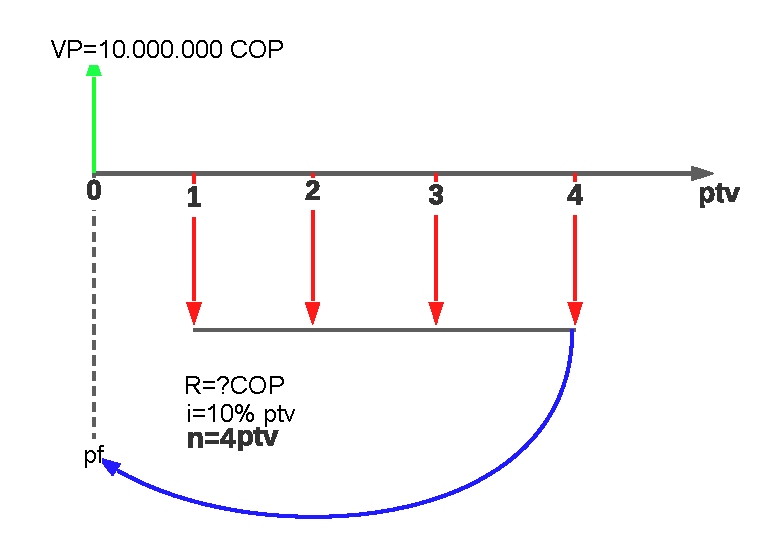
\includegraphics[scale=1]{4_Capitulo/img/ejemplos/9/capitulo4ejemplo9.pdf} } \\ \hline 
        %%%%%%%%%%%%% FIN INSERCIÓN DE IMAGEN
        %%%%%FIN FLUJO DE CAJA



        %%%%% INICIO DECLARACIÓN FORMULAS
        %%%%%%%%%%% INICIO TITULO
        \rowcolor[HTML]{FFB183}
        \multicolumn{3}{|c|}{\cellcolor[HTML]{FFB183}\textbf{4. Declaración de fórmulas}}       \\ \hline
        %%%%%%%%%%% FIN TITULO
        %%%%%%%%%%% INICIO MATEMÁTICAS

        \multicolumn{3}{|c|}{$VP=R\frac{(1-(1+i)^{-n})}{i}$ Valor presente serie uniforme vencida}  \\ \hline
        %%%%%%%%%% FIN MATEMÁTICAS
        %%%%%% INICIO DESARROLLO MATEMÁTICO
        \rowcolor[HTML]{FFB183}
        %%%%%%%%%%INICIO TITULO
        \multicolumn{3}{|c|}{\cellcolor[HTML]{FFB183}\textbf{5. Desarrollo matemático}}    \\ \hline
        %%%%%%%%%% FIN TITULO
        %%%%%%%%%% INICIO MATEMÁTICAS
        \multicolumn{3}{|c|}{10.000.000 COP$=R\frac{(1-(1+0,1)^{-4})}{0,1}$ }     \\ \hline
        %%%%%%%%%% FIN MATEMÁTICAS
        %%%%%% FIN DESARROLLO MATEMÁTICO

        \rowcolor[HTML]{FFB183}
        \multicolumn{3}{|c|}{\cellcolor[HTML]{FFB183}\textbf{6. Respuesta}}    \\ \hline

        \multicolumn{3}{|c|}{R=3.154.708 COP} \\ \hline
        \multicolumn{3}{|c|}{ 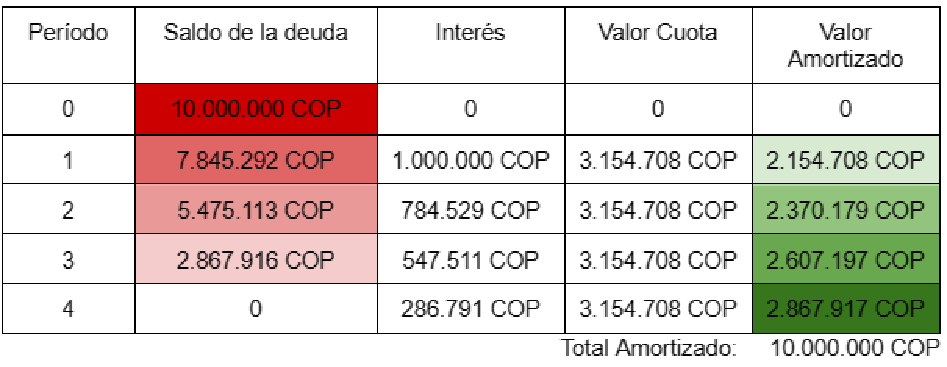
\includegraphics[scale=0.8]{4_Capitulo/img/ejemplos/9/Capitulo4Ejemplo9Solucion.pdf} } \\ \hline      
    \end{longtable}
    %Se crean dos lineas en blanco para que no quede el siguiente texto tan pegado
    %\newline \newline
\end{center}
%%%%%%%%%%%%%%%%%%%%%%%%%%FIN EJERCICIO X %%%%%%%%%%%%%%%%%%%%%%%%%%%
